\begin{figure*}[t]
\providecommand{\width}{}
\renewcommand{\width}{0.15\textwidth}
\centering
\begin{subfigure}[t]{\width}
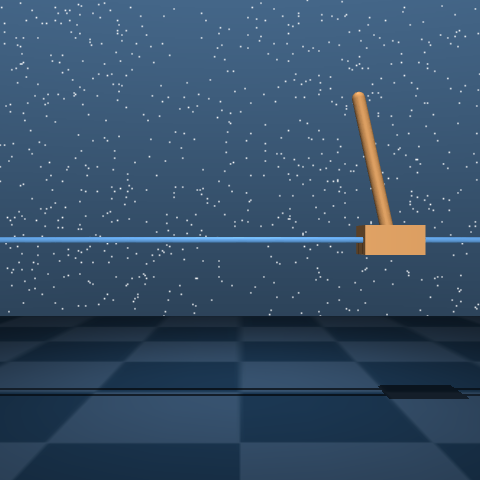
\includegraphics[width=\textwidth]{figures/domains/cartpole}
\caption{Cartpole}
\end{subfigure}\hfill%
\begin{subfigure}[t]{\width}
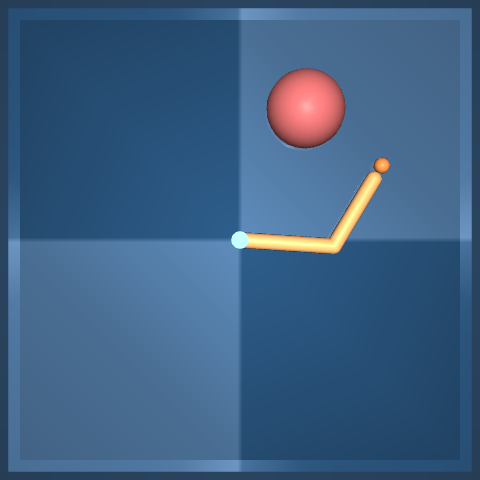
\includegraphics[width=\textwidth]{figures/domains/reacher}
\caption{Reacher}
\end{subfigure}\hfill%
\begin{subfigure}[t]{\width}
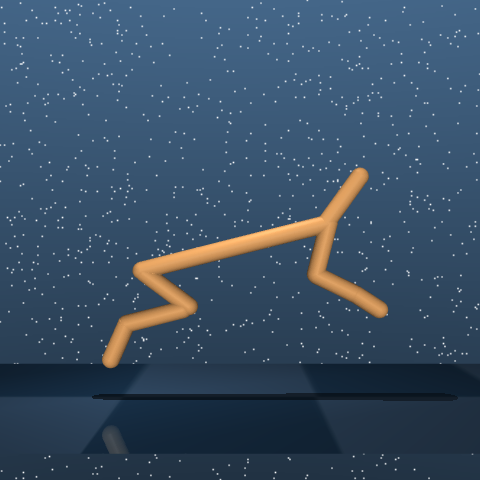
\includegraphics[width=\textwidth]{figures/domains/cheetah}
\caption{Cheetah}
\end{subfigure}\hfill%
\begin{subfigure}[t]{\width}
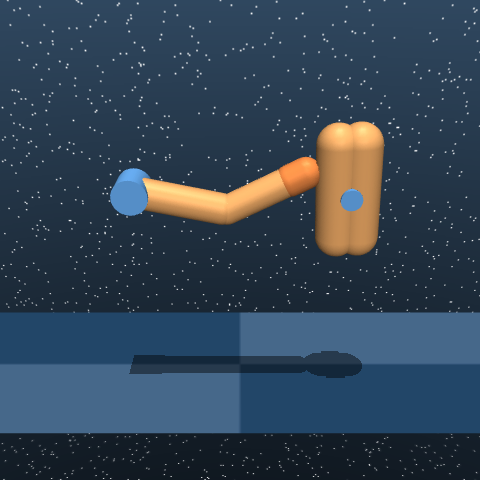
\includegraphics[width=\textwidth]{figures/domains/finger}
\caption{Finger}
\end{subfigure}\hfill%
\begin{subfigure}[t]{\width}

\includegraphics[width=\textwidth]{figures/domains/cup}
\caption{Cup}
\end{subfigure}\hfill%
\begin{subfigure}[t]{\width}

\includegraphics[width=\textwidth]{figures/domains/walker}
\caption{Walker}%
\end{subfigure}%
\caption{实验中使用的基于图像的控制域。图像展示的是缩放到 $64\times 64\times 3$ 像素之前的智能体观测。(a) Cartpole swingup 任务使用固定相机，因此小车可能移出视野。(b) Reacher 任务只有稀疏奖励。(c) Cheetah running 任务包含接触动力学和更多关节。(d) Finger spinning 任务包含手指与物体之间的接触。(e) Cup 任务奖励稀疏，只有接住球后才给出奖励。(f) Walker 任务要求机器人在倒地后保持平衡，并预测与地面之间较复杂的相互作用。}
\label{fig:domains}
\end{figure*}
